% ============================ Enrico Ribiani 16-03-2021 ====================================================================
% Base per i documenti  
\documentclass[12pt]{article}
% ------------ pacchetti necessari ----------------
\usepackage[a4paper, total={6in, 8in},margin=1in]{geometry} % formattazione decente della pagina
\usepackage{graphicx}                            % need for figure
\usepackage{amsmath}
\usepackage{amsfonts}                            % if you want the fonts
\usepackage{amssymb}                             % if you want extra symbols
\usepackage{graphicx}  
\renewcommand{\figurename}{Figura}  
\renewcommand{\contentsname}{Indice}                        % need for figures
\usepackage{mathptmx}
\usepackage{float}                               % serve per mettere tabelle e immagini dove si vuole 
\usepackage[utf8]{inputenc}
\usepackage{textcomp}
\usepackage[hang,flushmargin,bottom]{footmisc}   % footnote format
\usepackage{fancyhdr, lastpage}
\usepackage{titlesec}
\usepackage[table,dvipsnames]{xcolor}
%\pagestyle{fancy}
%\renewcommand{\headrulewidth}{0pt}
%\renewcommand*\contentsname{Indice}
\titleformat{\section}{\normalsize\bfseries}{\thesection.}{1em}{}	% required for heading numbering style
\titleformat*{\section}{\Large\bfseries}
\titleformat*{\subsection}{\large\bfseries}
%\usepackage{siunitx}
%\usepackage{tikz}
\usepackage{circuitikz}
\usepackage{multicol}
%\usepackage[siunitx]{circuitikz}
\usepackage{multirow}
\usepackage{tikz}
\usepackage{amsmath}
\usetikzlibrary{angles,quotes}
\usepackage{placeins}
\usepackage{pdfpages}
\usepackage{wrapfig}
\usepackage{wasysym}
%===================links=================
\usepackage{hyperref}
\hypersetup{
    colorlinks=true,
    linkcolor=darkgray,
    filecolor=Green,      
    urlcolor=Cyan,
    pdftitle={relazione-elt},
    pdfpagemode=FullScreen,
    }

%===================inizio pagina del titolo=================
\begin{document}
    \begin{titlepage}
    \begin{center}
% ------------------ inizio immagine logo ----------
\begin{figure}
    \centering
    \includegraphics[scale=1.5]{Logo.png}
    \label{fig:logo}
\end{figure}
% ------------------ fine immagine logo ----------
% ------------------ fine immagine logo ----------
-------------------------------------------------------------------------------------\\
\vspace{2\baselineskip}
\large Prova n°4
\hfill
\large $5^a$   AUB\\
\begin{flushleft}
    \large Enrico Ribiani\\
    \large Daniel Graziadei\\
    %\large Gruppo 11\\
\end{flushleft}


\vfill

\Huge{\textbf{Regolatore}}\\
\vfill
\vfill
\large{12-01-2023}
\end{center}
%=============== fine pagina titolo ===============
\end{titlepage}
\tableofcontents
\newpage
\vskip 1cm
\section{Scopo}
In questa esperienza verificheremo sperimentalmente il comportamento di due regolatori integrati:\\
- \textit{L7812} con varie resistenze\\
- \textit{LM317}
La verifica dei valori verrà effettuata tramite misure di tensione e corrente.\\
\noindent
    \section{Schemi} 
\begin{figure}[!h]
    \centering
    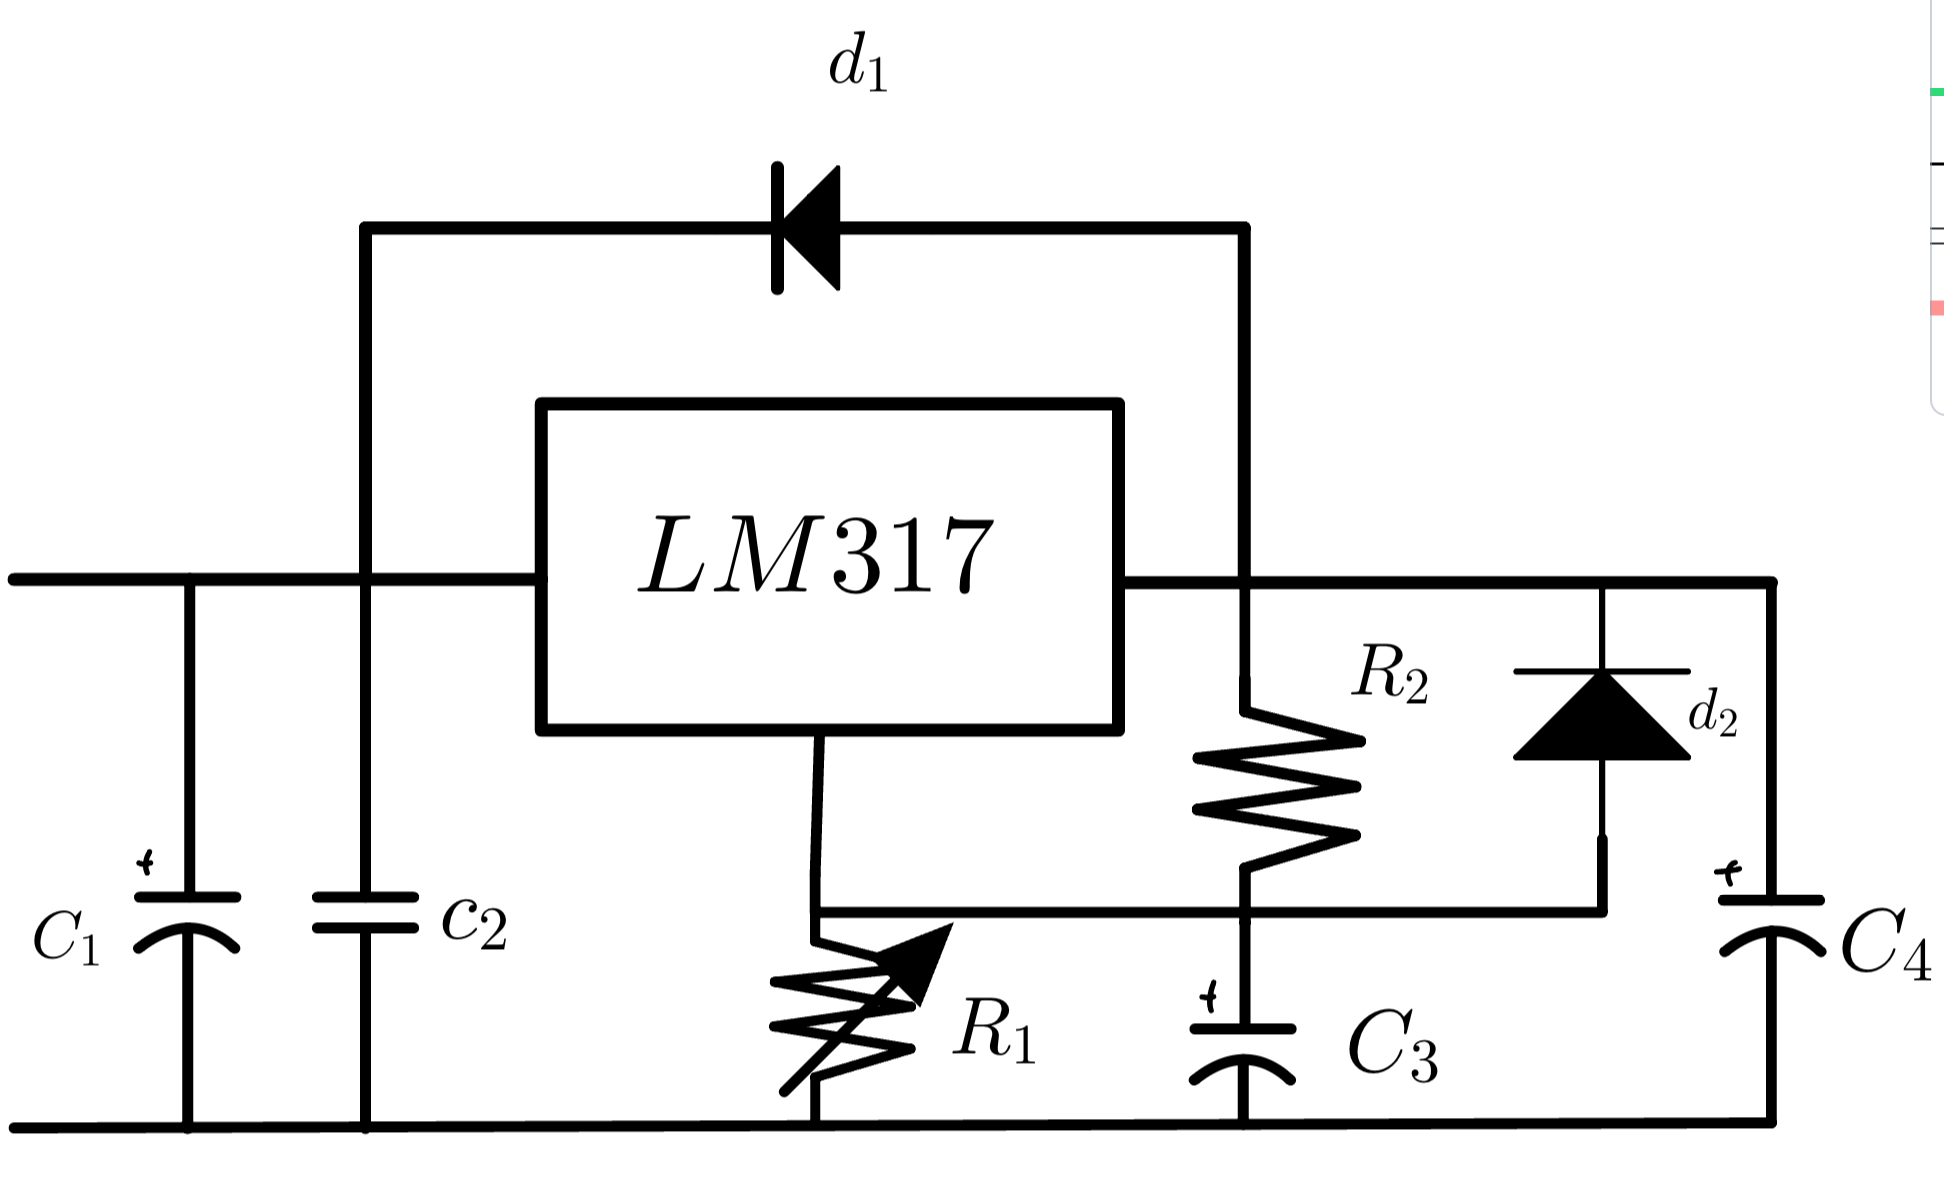
\includegraphics[scale=0.1]{schema.jpg}
    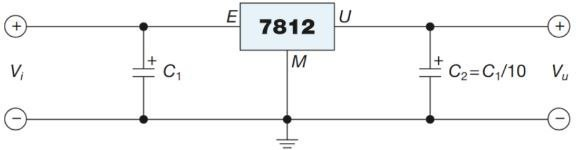
\includegraphics[scale=0.4]{schema2.jpg}
    %\caption{Caption}
    %\label{fig:my_label}
\end{figure}
    \section{Materiale e Strumenti}
    \begin{multicols}{2}
    \begin{itemize}
    \item Fili di collegamento
    \item Breadboard
    \item Resistenza da $200\Omega$
    \item Potenziometro da $660\Omega$
    \item 3x Condensatore elettrolitico da $100\mu$F
    \item Condensatore da $10\mu$F
    \item \textit{LM317}
    \item 2x Diodi
    \end{itemize}
    \vfill\null
    \columnbreak
    \begin{itemize}
    \item Multimetro
    \item Alimentazione DC 
    \end{itemize}
    \vfill\null
    \end{multicols}
    \section{Contenuti teorici}
    I componenti del circuito LM317 sono i seguenti:\\
    \begin{itemize}
        \item C1, condensatore elettrolitico avente la funzione di compensare le induttanze parassite dei conduttori
        tramite i quali viene applicata la tensione da stabilizzare all’ingresso del regolatore.
        \item C2, condensatore in poliestere o ceramico, collegato tra il terminale d’ingresso (E) e la massa, per 
        evitare auto-oscillazioni dell’integrato.
        \item C3, condensatore elettrolitico, che stabilizza la tensione sul terminale di regolazione (R).
        \item C4, condensatore elettrolitico connesso sul terminale di uscita (U), con la funzione di eliminare eventuali
        residui di corrente alternata.
        \item D1, diodo posto tra l’uscita e l’ingresso, avente la funzione di proteggere l’integrato ogni volta che si 
        spegne il regolatore: infatti, senza questo diodo, il condensatore C4 si scaricherebbe in senso inverso all’interno
        dell’integrato, cioè dall’uscita verso l’ingresso, con il rischio di danneggiare l’integrato stesso.
        \item D2, diodo collegato tra i terminali R e U, avente la funzione di scaricare il condensatore C3 in caso di 
        cortocircuito accidentale sui terminali d’uscita (e causare danni).
        \item R1, resistenza di valore fisso pari a 220 $\Omega$ (1/4 W), che insieme a R2 realizza un partitore resistivo dal quale viene
        prelevata la tensione da applicare al terminale R di regolazione.
        \item R2, resistenza il cui valore deve essere determinato in funzione della tensione stabilizzata che si vuole ottenere in
        uscita.\\
    \end{itemize}  

    \noindent

    Invece l'integrato \textit{L7812} ha:\\
    Un dissipatore di calore in metallo collegato al piedino centrale
    \begin{itemize}
        \item E ingresso, tensione da stabilizzare
        \item E ingresso, tensione da stabilizzare
        \item M massa
        \item C1(elettrolitico): compensazione induttanze parassite dei conduttori
        \item C2(elettrolitico): migliorare la stabilità della tensione d’uscita mediante azione filtrante passa basso
    \end{itemize}
        \subsection{Descrizione della prova}
        Prima di tutto si monta il circuito come da schema su breadboard usando il regolatore 7812 consultando il 
        datasheet per capire i pin di entrata, uscita e massa.\\ Dopo di che si alimenta il circuito mettendo i cavi 
        dell'alimentatore ai capi di C1 facendo attenzione a mettere al minimi tensione e corrente.\\ Successivamente si 
        passa alla presa dei dati, ovvero con un multimetro collegato ai capi di C2 si misura la tensione d'uscita ad 
        ogni valore di tensione d'entrata con ogni resistenza.\\ Infine si calcola la corrente d'uscita dividendo la 
        tensione d'uscita con la resistenza usata.\\
        Lo stesso procedimento si fa con LM317, si monta il circuito e lo si alimenta mettendo i cavi ai capi di C1, 
        ad ogni valore di tensione d'entrata ci si appunta il corrispondente valore di uscita.\\
        \subsection{Raccolta dei dati}
    \noindent
        
    \begin{figure}[p]
            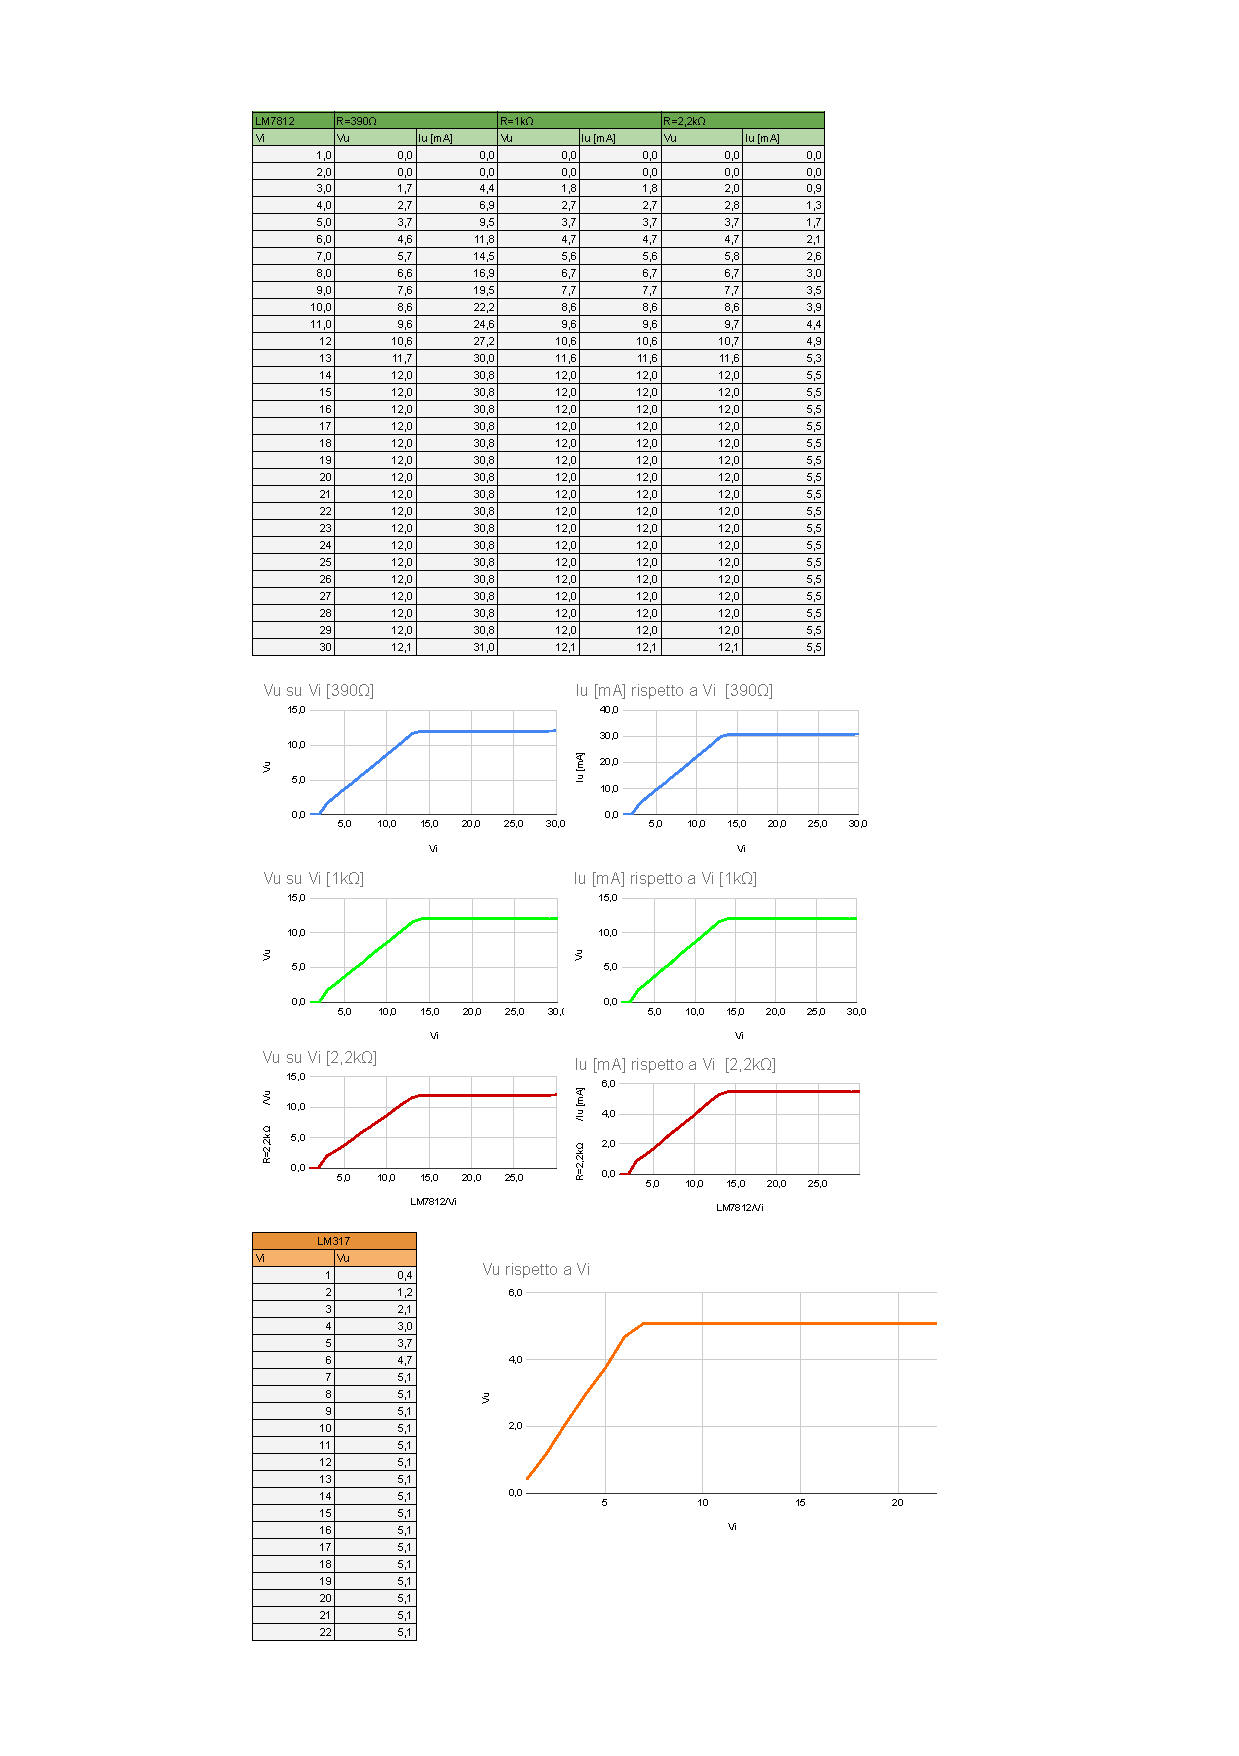
\includegraphics[scale=0.9]{tab.pdf}
            %\caption{}
           % \label{fig:my_label}
        \end{figure}
        \subsection{Commento dei dati raccolti}
        Dalle tabelle si può vedere come i dispostivi regolano l’uscita solo da un certo valore di tensione d’ingresso.\\
        Nel \textit{L7812} si può notare come l’uscita si stabilizza dai 14 V di entrata, mentre al \textit{LM317} ne 
        bastano 7.\\
        Questo si può confermare guardando il datasheet dei componenti.\\
        Nel 7812 si può osservare come la tensione d’uscita cambia quando si varia il valore della resistenza.\\
        Con una resistenza minore si ha una maggiore Vout mentre con una resistenza maggiore si ha una minore Vin.\\

        \subsection{Calcoli}
        $V_{ref}=V_u\cdot \frac{R_1}{R_1+R_2}=1,25\cdot \frac{6,5}{220+R}$ da cui $R=770\Omega$
    \section{Analisi critica dei risultati e conclusioni}
    I dati raccolti sperimentalmente esposti in tabella e analizzati tramite  i grafici di tensione
    e corrente corrispondono ai risultati aspettati dall'esperienza infatti i entrambi i regolatori
    possiamo notare la crescita della tensione e della correnta fino a un determinato valore in cui
    si stabilizzano i valori.\\
    Si può inoltre notare nel caso del regolatore \textit{LM317} come i valori di corrente cambiano
    utilizzando vari valori di resistenza.\\
%-----------------------------------------

\end{document}